\chapter{Estrazione del Segnale ECG tramite Segmentazione Semantica}

Il presente capitolo descrive il modulo \texttt{ecg-signal-extractor}, che implementa la pipeline di addestramento di un modello di segmentazione semantica per l'estrazione dei tracciati ECG utilizzando le immagini prodotte dal generatore. Il modulo costituisce il secondo stadio della pipeline complessiva e supporta due modalità operative: addestramento su immagini già augmentate (\texttt{--base\_dir\_augmented}) e addestramento con augmentation generata al volo a partire da immagini pulite (\texttt{--base\_dir}).

\section{Obiettivo e Collocazione nel Progetto}

Il generatore descritto nei capitoli precedenti produce immagini ECG sintetiche realistiche accompagnate dalla corrispondente ground truth visiva: un'immagine binaria in cui i pixel bianchi rappresentano esclusivamente i tracciati del segnale, senza griglia né artefatti. Questa coppia costituisce l'input ideale per addestrare un modello di \textit{segmentazione semantica}, il cui obiettivo è apprendere la mappatura inversa: data un'immagine ECG con tutti i suoi artefatti, produrre una maschera binaria che individui i pixel appartenenti al tracciato.

Il task è intrinsecamente difficile per tre ragioni. In primo luogo, i tracciati ECG sono strutture sottili, spesso di pochi pixel di spessore, disperse su un'area molto estesa; una piccola imprecisione della maschera predetta si traduce in un errore sistematico nella ricostruzione numerica del segnale. In secondo luogo, la griglia millimetrata condivide alcune caratteristiche visive con i tracciati (linee sottili, orientamento misto orizzontale-verticale), rendendo la discriminazione non banale. In terzo luogo, gli artefatti applicati dal generatore — pieghe, testo manoscritto, rumore fotometrico — modificano localmente l'aspetto del segnale, richiedendo che il modello sia robusto a una vasta gamma di condizioni degradate.

\section{Architettura del Modello}

\subsection{U-Net con Encoder Pre-addestrato}

Il modello adottato è una \textbf{U-Net}~\cite{ronneberger2015unetconvolutionalnetworksbiomedical}, l'architettura di riferimento per la segmentazione semantica di immagini biomedicali. La U-Net è una rete encoder-decoder completamente convoluzionale caratterizzata da connessioni skip che collegano ogni livello dell'encoder al corrispondente livello del decoder: queste connessioni trasmettono direttamente le feature maps ad alta risoluzione dell'encoder al decoder, permettendo a quest'ultimo di recuperare i dettagli spaziali fini che si perderebbero durante la progressiva riduzione di risoluzione.

\begin{figure}[H]
    \centering
    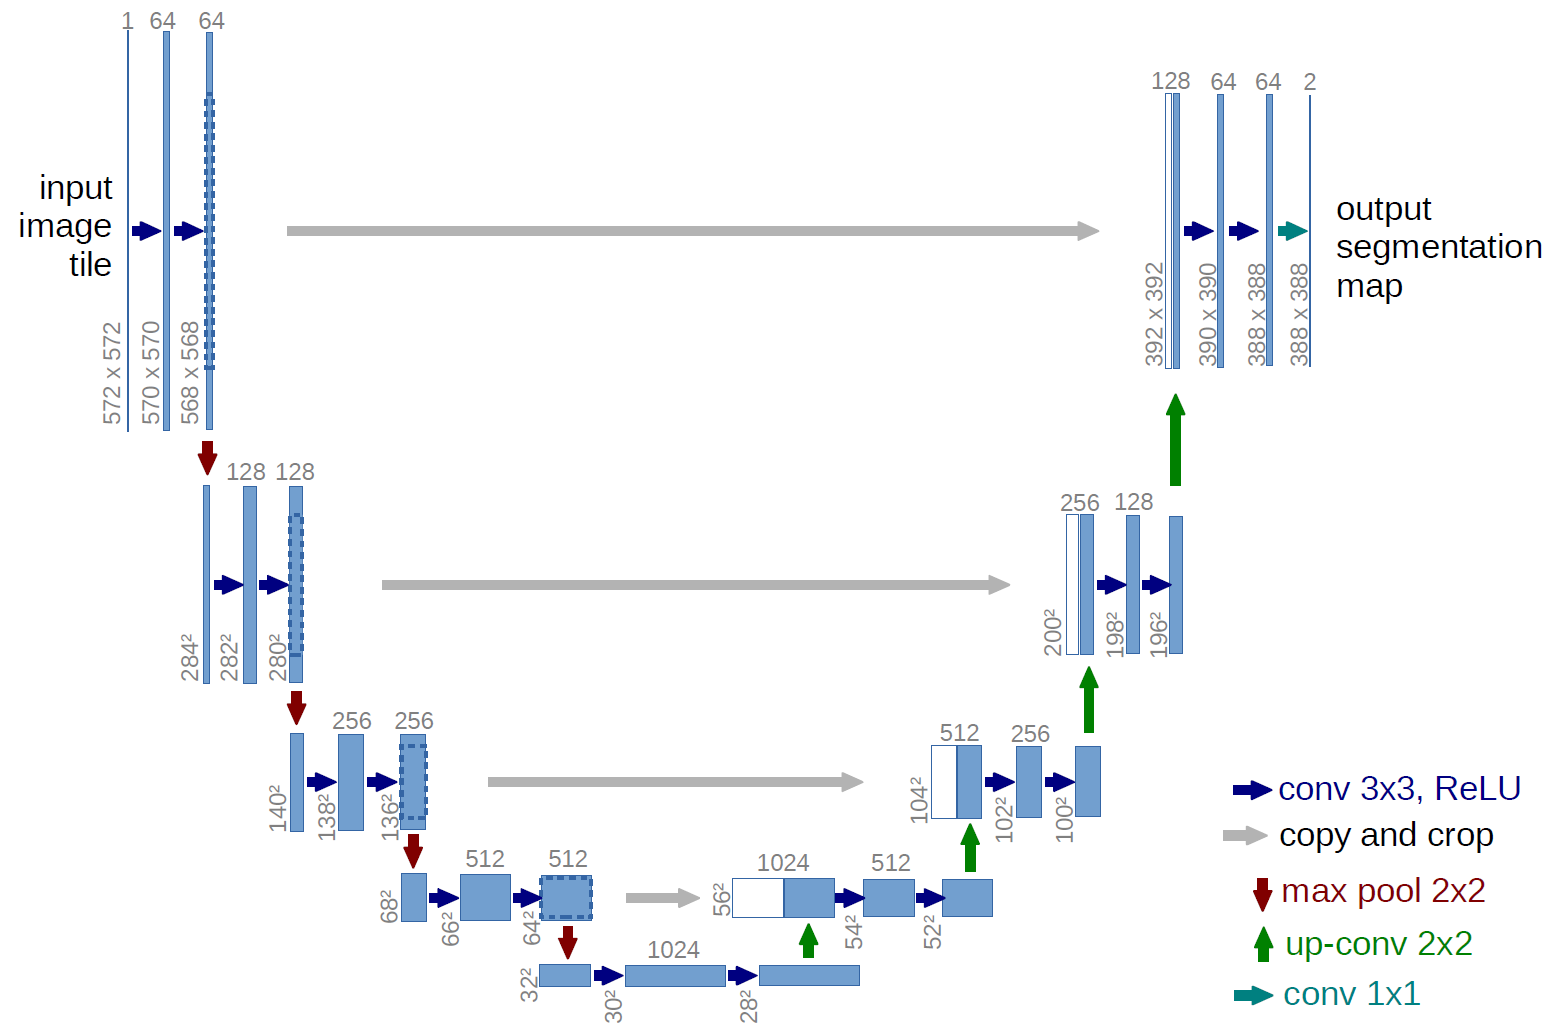
\includegraphics[width=0.85\textwidth]{images/u-net-architecture.png}
    \caption{Architettura U-Net originale~\cite{ronneberger2015unetconvolutionalnetworksbiomedical}. Il percorso di contrazione (sinistra) riduce progressivamente la risoluzione spaziale tramite max pooling estraendo feature maps sempre più astratte; il percorso di espansione (destra) ricostruisce la risoluzione originale tramite up-convolution. Le frecce grigie rappresentano le connessioni skip che copiano le feature maps dall'encoder al decoder.}
    \label{fig:unet_architecture}
\end{figure}

L'implementazione utilizza la libreria \texttt{segmentation-models-pytorch}~\cite{Iakubovskii:2019} tramite la classe \texttt{smp.Unet}, configurata con i seguenti parametri fissi:

\begin{itemize}
    \item \textbf{Canali di ingresso:} 3 (immagine RGB).
    \item \textbf{Classi di output:} 1 (segmentazione binaria: tracciato vs.\ sfondo).
    \item \textbf{Tipo di attenzione nel decoder:} \texttt{scse} (Squeeze-and-Excitation concorrente).
    \item \textbf{Encoder:} configurabile tramite \texttt{--encoder}; default \texttt{resnet50}, con pesi pre-addestrati su ImageNet.
\end{itemize}

L'encoder è intercambiabile: architetture CNN classiche come \texttt{resnet50} \cite{he2015deepresiduallearningimage} ed \texttt{efficientnet-b5} offrono un buon equilibrio tra precisione e consumo di VRAM, mentre backbone transformer come \texttt{mit-b4} (Mix Transformer~\cite{xie2021segformersimpleefficientdesign}) forniscono maggiore capacità di modellare dipendenze a lungo raggio al costo di un consumo di memoria superiore.

\subsection{Decoder con Attenzione scSE}

Il decoder è dotato di un meccanismo di \textbf{attenzione scSE} (\textit{Concurrent Spatial and Channel Squeeze \& Excitation})~\cite{roy2018concurrentspatialchannelsqueeze}, che permette alla rete di filtrare automaticamente le informazioni meno utili prima di produrre la maschera finale. Il blocco opera in parallelo su due dimensioni distinte delle feature maps:

\begin{itemize}
    \item \textbf{Attenzione per canale (cSE):} Ogni strato di una feature map rappresenta un diverso tipo di caratteristica visiva appresa dall'encoder (bordi, texture, variazioni di intensità, ecc.). Il blocco cSE esegue una \textit{global average pooling} sull'intera mappa spaziale per ottenere un vettore riassuntivo, lo elabora attraverso due layer fully-connected e produce un peso per ciascun canale. Questi pesi vengono moltiplicati per le feature maps originali, amplificando le caratteristiche più discriminative per la segmentazione dei tracciati e sopprimendo quelle meno rilevanti.
    \item \textbf{Attenzione spaziale (sSE):} Invece di ragionare sui tipi di caratteristiche, il blocco sSE si chiede \textit{dove} si trovano le informazioni importanti. Applica una convoluzione $1\times1$ che collassa tutti i canali in un singolo valore per pixel, ottenendo una mappa di attenzione spaziale. Questa mappa viene moltiplicata per le feature maps originali, in modo che le regioni occupate dal tracciato vengano enfatizzate e quelle di griglia o sfondo attenuate.
\end{itemize}

I due output vengono sommati, combinando la risposta a \textit{cosa guardare} (cSE) con quella a \textit{dove guardare} (sSE). Per strutture sottili e allungate come i tracciati ECG — che occupano una piccola frazione dei pixel totali e condividono caratteristiche visive con la griglia — questa doppia ricalibrazione è particolarmente efficace nel ridurre i falsi positivi sulla griglia millimetrata.

\begin{figure}[H]
    \centering
    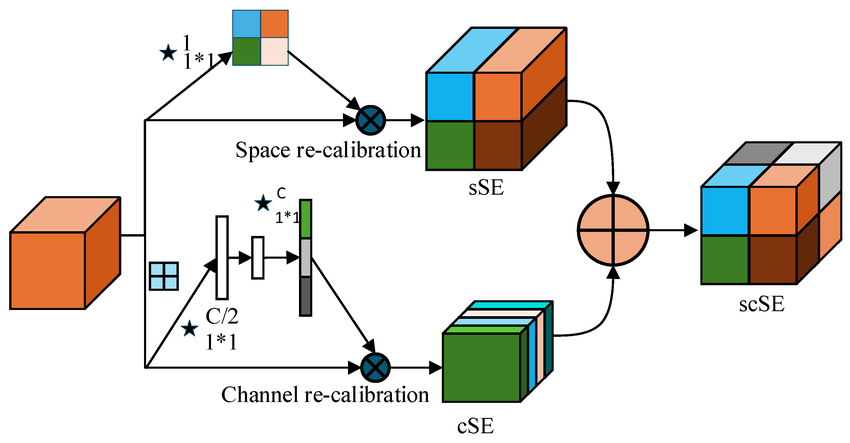
\includegraphics[width=0.75\textwidth]{images/scSE.png}
    \caption{Schema del blocco scSE~\cite{roy2018concurrentspatialchannelsqueeze}. Il ramo superiore (sSE) applica una convoluzione $1\times1$ per produrre la mappa di attenzione spaziale; il ramo inferiore (cSE) comprime la dimensione spaziale e ricalibra i canali tramite due convoluzioni $1\times1$. I due output vengono sommati elemento per elemento.}
    \label{fig:scse}
\end{figure}

\subsection{Funzione di Perdita Composita}

La funzione di perdita è la somma di tre contributi complementari, ciascuno progettato per correggere un diverso tipo di errore di segmentazione:

\[
    \mathcal{L} = w_{\text{focal}}\,\mathcal{L}_{\text{Focal}} + w_{\text{dice}}\,\mathcal{L}_{\text{Dice}} + w_{\text{cl}}\,\mathcal{L}_{\text{clDice}}
\]

I pesi $w$ vengono adattati ai tre stage di addestramento descritti nella Sezione~\ref{sec:curriculum}: il peso della clDice Loss aumenta progressivamente man mano che le immagini diventano più difficili, per penalizzare sempre di più le interruzioni nei tracciati in presenza di artefatti pesanti. I pesi di Focal e Dice rimangono invece costanti.

\subsubsection{Focal Loss}

La Focal Loss~\cite{lin2018focallossdenseobject} affronta un problema fondamentale di questo task: i pixel di tracciato sono una minoranza estrema dell'immagine (meno del 5\% del totale), e una loss standard come la Binary Cross-Entropy tenderebbe a ignorarli, imparando semplicemente a classificare tutto come sfondo.

La Focal Loss risolve questo sbilanciamento modulando il peso di ogni pixel in base alla difficoltà della sua classificazione. I pixel già classificati correttamente con alta confidenza contribuiscono poco al gradiente; quelli difficili — come i pixel di tracciato parzialmente oscurati da un artefatto — ricevono un peso maggiore e guidano l'apprendimento. Formalmente:

\[
    \mathcal{L}_{\text{Focal}} = -\frac{1}{N}\sum_i \bigl[\alpha_t\,(1-p_t)^\gamma \cdot \log(p_t)\bigr]
\]

dove $p_t$ è la probabilità predetta per la classe corretta del pixel $i$, $\gamma = 2.0$ è il fattore di modulazione che controlla quanto penalizzare i pixel facili, e $\alpha_t$ è il fattore di bilanciamento per classe ($\alpha = 0.8$ per i pixel di tracciato, $1-\alpha = 0.2$ per lo sfondo).

\subsubsection{Dice Loss}

Mentre la Focal Loss opera pixel per pixel, la Dice Loss~\cite{sudre2017generalised} valuta la qualità della maschera complessiva misurando la sovrapposizione tra la maschera predetta e la ground truth. Il suo valore è 0 quando le due maschere coincidono perfettamente e 1 quando non hanno nessun pixel in comune:

\[
    \mathcal{L}_{\text{Dice}} = 1 - \frac{2 \sum_i p_i g_i}{\sum_i p_i + \sum_i g_i}
\]

dove $p_i$ è la probabilità predetta per il pixel $i$ e $g_i$ è il valore della ground truth ($0$ o $1$). La Dice Loss è intrinsecamente insensibile allo sbilanciamento tra classi, perché si normalizza rispetto al numero di pixel positivi, non al totale. La combinazione con la Focal Loss è consolidata nella letteratura di segmentazione biomedicale~\cite{isensee2021nnunet}: la Focal Loss guida la rete verso i pixel difficili, mentre la Dice Loss garantisce che la forma complessiva della maschera sia corretta.

\subsubsection{centerline Dice Loss}

Anche una maschera con ottima Focal e Dice Loss può essere inutilizzabile in pratica: basta una piccola lacuna nel tracciato predetto — un gruppo di pixel classificati erroneamente come sfondo — per interrompere la continuità del segnale e rendere impossibile la successiva ricostruzione numerica. Dice e Focal ottimizzano la correttezza pixel per pixel, ma non penalizzano queste interruzioni topologiche.

La \textbf{centerline Dice Loss} ($\mathcal{L}_{\text{clDice}}$), introdotta da Shit et al.~\cite{Shit_2021} per strutture tubulari e filiformi, risolve questo problema confrontando non le maschere intere, ma i loro \textit{scheletri}: la linea centrale di un pixel di spessore che ne descrive la topologia. Se la maschera predetta ha una lacuna, il suo scheletro è interrotto nel punto corrispondente, e questa interruzione produce un penalità elevata.

Poiché la scheletrizzazione morfologica classica non è differenziabile e non può essere usata in un ciclo di backpropagation, la clDice utilizza un \textit{soft skeleton} $\mathcal{S}(M)$, una versione continua e derivabile ottenuta iterando composizioni di erosione e dilatazione morbida (realizzate tramite max-pooling):

\[
    \mathcal{S}^{(0)}(M) = \mathrm{ReLU}\!\left(M - \widetilde{\mathcal{O}}(M)\right), \qquad
    \mathcal{S}^{(t)}(M) = \mathcal{S}^{(t-1)}(M) + \mathrm{ReLU}\!\left(\delta^{(t)} - \mathcal{S}^{(t-1)}(M)\cdot\delta^{(t)}\right)
\]

dove $\widetilde{\mathcal{O}} = \widetilde{\mathcal{D}} \circ \widetilde{\mathcal{E}}$ è l'apertura morbida e $\delta^{(t)}$ è il contributo dell'iterazione $t$. L'implementazione utilizza 15 iterazioni: un numero maggiore permette allo scheletro di propagarsi lungo porzioni più estese del tracciato, rendendo la perdita sensibile anche alle interruzioni lontane dagli estremi della linea. La loss è definita come:

\[
    \mathcal{L}_{\text{clDice}} = 1 - \frac{2 \cdot T_{\text{prec}} \cdot T_{\text{sens}}}{T_{\text{prec}} + T_{\text{sens}}}
\]

con

\[
    T_{\text{prec}} = \frac{\sum_i \mathcal{S}(\hat{p})_i \cdot g_i + \epsilon}{\sum_i \mathcal{S}(\hat{p})_i + \epsilon}, \qquad
    T_{\text{sens}} = \frac{\sum_i \mathcal{S}(g)_i \cdot \hat{p}_i + \epsilon}{\sum_i \mathcal{S}(g)_i + \epsilon}
\]

dove $\hat{p} = \sigma(\text{logits})$ è la predizione dopo sigmoid e $\epsilon = 1$ è un termine di smoothing. $T_{\text{prec}}$ misura quanta parte dello scheletro predetto coincide con la ground truth (lo scheletro è nel posto giusto?), mentre $T_{\text{sens}}$ misura quanta parte dello scheletro della ground truth è coperta dalla predizione (nessuna parte del tracciato reale è stata persa?). Se la ground truth è vuota, il termine clDice viene saltato per evitare gradienti instabili su maschere nulle.

\section{Modalità Operative}

Il modulo supporta due modalità di addestramento, selezionate tramite argomenti mutuamente esclusivi.

\subsection{Modalità con Augmentation al Volo (\texttt{--base\_dir})}

Nella modalità \texttt{--base\_dir} il dataset è una cartella piatta contenente coppie immagine pulita / maschera ground truth. La classe \texttt{ECGBaseDataset} carica l'immagine pulita come base e, durante il training, applica ad ogni iterazione una trasformazione casuale tramite le funzioni \texttt{get\_augment()} e \texttt{get\_creased()} del modulo \texttt{ecg-image-generator}. La maschera subisce le stesse trasformazioni geometriche (rotazione) in modo sincronizzato.

\begin{figure}[H]
\raggedright
\begin{dirtree}{%
.1 <base\_dir>/.
.2 record\_001.png \DTcomment{immagine pulita (base per augmentation)}.
.2 record\_001\_clean.png \DTcomment{maschera ground truth}.
.2 record\_002.png.
.2 record\_002\_clean.png.
.2 \ldots.
}
\caption{Struttura attesa del dataset nella modalità \texttt{--base\_dir}.}
\label{fig:extractor_basedir}
\end{dirtree}
\end{figure}

Il dataset viene suddiviso automaticamente in training, validation e test con proporzione \textbf{80/10/10} tramite un seed fisso (42~\cite{adams1984hitchhiker}). Il percorso all'installazione del generatore viene specificato tramite \texttt{--generator\_path}, che viene aggiunto a \texttt{sys.path} sia nel processo principale che nei worker del DataLoader.

\paragraph{Parametri di augmentation al volo.} I parametri di augmentation vengono passati come limiti superiori; il valore effettivo applicato ad ogni immagine è campionato uniformemente nell'intervallo $[0, \text{max}]$, rispecchiando il comportamento del generatore. I principali parametri includono: rotazione massima (\texttt{--rotate}), blur gaussiano (\texttt{--blur}), dropout di sfondo (\texttt{--dropout}), rumore sale e pepe (\texttt{--salt\_pepper}), rumore gaussiano (\texttt{--gaussian\_noise}), compressione JPEG (\texttt{--jpeg\_compression}), fattore di luminosità (\texttt{--brightness}), temperatura del colore (\texttt{--temperature}), pieghe verticali/orizzontali (\texttt{--num\_creases\_vertically}, \texttt{--num\_creases\_horizontally}) e rughe (\texttt{--wrinkles}).

Quando \texttt{--temperature} è non zero, la temperatura viene randomizzata per ogni immagine tra 2000–4000 K (tono caldo) o 10000–20000 K (tono freddo), scelti con probabilità equiprobabili; il valore 0 seleziona una temperatura neutra di 6500 K senza alcuna variazione visibile.

\subsection{Modalità con Immagini Pre-augmentate (\texttt{--base\_dir\_augmented})}

Nella modalità \texttt{--base\_dir\_augmented} il dataset è già organizzato in tre sottodirectory di stage. La classe \texttt{ECGSegmentationDataset} esegue il caricamento senza alcuna augmentation aggiuntiva, applicando solo normalizzazione e ridimensionamento opzionale.

\begin{figure}[H]
\raggedright
\begin{dirtree}{%
.1 <base\_dir\_augmented>/.
.2 stage0\_easy/.
.3 record\_001.png.
.3 record\_001\_clean.png.
.3 \ldots.
.2 stage1\_medium/.
.3 \ldots.
.2 stage2\_hard/.
.3 \ldots.
}
\caption{Struttura attesa del dataset nella modalità \texttt{--base\_dir\_augmented}.}
\label{fig:extractor_augdir}
\end{dirtree}
\end{figure}

La divisione train/val/test viene calcolata una sola volta dal primo stage disponibile (seed 42) e applicata identicamente a tutti gli stage, in modo che gli stessi record appaiano negli stessi subset attraverso tutti gli stage. I parametri \texttt{--val\_split} (default: 0.1) e \texttt{--test\_split} (default: 0.1) controllano le proporzioni.

\subsection{Preprocessamento Comune}

Indipendentemente dalla modalità, il preprocessing finale di ogni immagine segue i passaggi:

\begin{enumerate}
    \item \textbf{Resize opzionale:} ridimensionamento a risoluzione quadrata configurabile tramite \texttt{--resize}. Le immagini vengono ridimensionate con interpolazione bilineare; per le maschere viene invece usata l'interpolazione \texttt{NEAREST}, che assegna a ogni pixel del risultato il valore del pixel più vicino nell'originale senza calcolare medie. Questo preserva la natura binaria della maschera: un'interpolazione bilineare produrrebbe valori intermedi (es. 0.3, 0.7) ai bordi del tracciato, che dopo la binarizzazione introdurrebbero artefatti lungo i contorni.
    \item \textbf{Normalizzazione} (\texttt{A.Normalize}): ogni canale RGB viene normalizzato sottraendo la media e dividendo per la deviazione standard calcolate sull'intero dataset ImageNet ($\mu = [0.485, 0.456, 0.406]$, $\sigma = [0.229, 0.224, 0.225]$). Questo passaggio è necessario perché i pesi pre-addestrati dell'encoder sono stati appresi su immagini normalizzate con questi stessi valori: presentare al modello immagini con una distribuzione diversa (pixel in $[0, 255]$ o $[0, 1]$) degraderebbe le feature estratte dall'encoder, vanificando il vantaggio del pre-addestramento.
    \item \textbf{Conversione a tensore} (\texttt{ToTensorV2}): l'array NumPy viene convertito in un tensore PyTorch riorganizzando le dimensioni dal layout \texttt{(H, W, C)} — altezza, larghezza, canali — al layout \texttt{(C, H, W)} atteso dai layer convoluzionali di PyTorch.
    \item \textbf{Binarizzazione della maschera:} i pixel della maschera con valore superiore a 10 (su scala 0–255) vengono impostati a 1.0, gli altri a 0.0. La soglia è volutamente bassa per recuperare anche i pixel di tracciato leggermente sbiaditi da eventuali artefatti fotometrici applicati alla ground truth. La maschera restituita ha shape \texttt{(1, H, W)}, dove la dimensione aggiuntiva rappresenta il singolo canale di output della segmentazione binaria.
\end{enumerate}

\section{Curriculum Learning}
\label{sec:curriculum}

\subsection{Motivazione}

Il \textit{curriculum learning}~\cite{10.1145/1553374.1553380} è una strategia di addestramento ispirata al processo pedagogico umano: il modello viene esposto prima agli esempi più semplici e progressivamente a quelli più complessi. Questa strategia è particolarmente efficace quando il dataset presenta una forte varianza di difficoltà, come nel caso delle immagini ECG sintetiche: un modello addestrato dall'inizio su immagini con tutti gli artefatti fatica a convergere, mentre uno che ha prima consolidato la struttura del segnale su immagini pulite generalizza meglio in seguito.

\subsection{Le Tre Fasi di Addestramento}

L'addestramento si articola in tre stage successivi di difficoltà crescente, processati nell'ordine \texttt{stage0\_easy} $\to$ \texttt{stage1\_medium} $\to$ \texttt{stage2\_hard}. Il modello non viene mai reinizializzato tra uno stage e il successivo.

\begin{table}[H]
\centering
\caption{Caratteristiche dei quattro stage di addestramento.}
\label{tab:extractor_stages}
\begin{tabular}{lllll}
\hline
\textbf{Stage} & \textbf{Epoche} & \textbf{LR default} & \textbf{Augmentation} & \textbf{Condizione} \\
\hline
\texttt{stage0\_easy}    & 20 (fisso)                      & \texttt{--lr} ($10^{-4}$)               & Nessuna      & sempre \\
\texttt{stage1\_medium}  & \texttt{--epochs} (default 100) & \texttt{--lr\_medium} ($10^{-5}$)       & Completa     & sempre \\
\texttt{stage2\_hard}    & \texttt{--epochs} // 2          & \texttt{--lr\_hard} ($10^{-6}$)         & Completa     & sempre \\
\texttt{det\_finetune}   & \texttt{--det\_finetune\_epochs} (default 30) & \texttt{--det\_finetune\_lr} ($10^{-3}$) & Completa & solo \texttt{--detection} \\
\hline
\end{tabular}
\end{table}

Nella modalità \texttt{--base\_dir}, la funzione \texttt{scale\_augment\_args()} disabilita tutta l'augmentation per lo stage 0 (blur, rumore, compressione JPEG, rotazione, pieghe e rughe vengono azzerati), lasciando al modello la possibilità di apprendere la struttura pulita del segnale senza interferenze. Gli stage 1 e 2 utilizzano la stessa intensità di augmentation completa, in modo che la progressione curricolare derivi dall'unfreezing progressivo dell'encoder, non da un cambio di distribuzione dei dati.

\subsection{Parametric Dropout per Stage}

Il dropout è una tecnica di regolarizzazione che durante il training disattiva casualmente una frazione dei neuroni ad ogni forward pass, forzando la rete a non dipendere da singoli percorsi di attivazione e a sviluppare rappresentazioni più robuste e ridondanti. La frazione di neuroni disattivati è controllata dal parametro $p$: un valore più alto corrisponde a una regolarizzazione più aggressiva.

In questo modulo, $p$ non è fisso ma viene aggiornato all'inizio di ogni stage secondo la formula:

\[
    p_{\text{dropout}} = 0.05 \times (\text{stage\_idx} + 1)
\]

ovvero 5\% nello stage 0, 10\% nello stage 1 e 15\% nello stage 2. La logica è che negli stage avanzati il modello riceve immagini con artefatti complessi e pattern di rumore molto specifici: senza una regolarizzazione sufficiente, rischierebbe di memorizzare quei pattern invece di generalizzare. Aumentare $p$ progressivamente forza la rete ad essere più robusta man mano che la difficoltà degli input cresce, senza però introdurre troppa regolarizzazione nelle fasi iniziali, quando il modello sta ancora imparando la struttura di base del segnale.

\subsection{Unfreezing Progressivo dell'Encoder (\texttt{--freeze\_encoder})}

Quando il flag \texttt{--freeze\_encoder} è attivo, i parametri dell'encoder vengono congelati e scongelati progressivamente attraverso gli stage, secondo lo schema seguente:

\begin{table}[H]
\centering
\caption{Stato dell'encoder per stage con \texttt{--freeze\_encoder}.}
\label{tab:extractor_freeze}
\begin{tabular}{ll}
\hline
\textbf{Stage} & \textbf{Stato dell'encoder} \\
\hline
\texttt{stage0\_easy}   & Completamente congelato \\
\texttt{stage1\_medium} & \texttt{layer3} e \texttt{layer4} scongelati \\
\texttt{stage2\_hard}   & Completamente scongelato \\
\hline
\end{tabular}
\end{table}

Questa strategia protegge i pesi ImageNet durante la fase iniziale (in cui il modello impara la struttura di base del segnale su immagini pulite), consentendo il fine-tuning specifico del dominio solo nelle fasi successive, quando il modello ha già sviluppato una rappresentazione stabile dei tracciati.

Durante il training, i layer \texttt{BatchNorm} dell'encoder vengono mantenuti in modalità \texttt{eval()} tramite la funzione \texttt{freeze\_bn()}, indipendentemente dallo stato di congelamento dei loro parametri.

I layer BatchNorm normalizzano le attivazioni di ogni layer durante il training usando la media e la varianza calcolate sul batch corrente, poi aggiornano delle statistiche globali (media e varianza mobili) che vengono usate in inferenza. Il problema è che queste statistiche sono già state calibrate su ImageNet durante il pre-addestramento: se le si lasciasse aggiornare su batch piccoli di immagini ECG — una distribuzione molto diversa da ImageNet — le stime risulterebbero rumorose e instabili, corrompendo le feature maps dell'encoder e degradando le performance. Mantenere il BatchNorm in modalità \texttt{eval()} congela le statistiche ai valori pre-addestrati, garantendo che l'encoder produca rappresentazioni coerenti anche quando i suoi parametri vengono aggiornati negli stage successivi.

\subsection{Scheduling del Learning Rate}

Il learning rate è specificato separatamente per i tre stage tramite i parametri \texttt{--lr}, \texttt{--lr\_medium} e \texttt{--lr\_hard} (default: $10^{-4}$, $10^{-5}$, $10^{-6}$). Questo approccio consente una riduzione aggressiva del learning rate attraverso gli stage per preservare la conoscenza acquisita — un fenomeno noto come \textit{catastrophic forgetting} — con la possibilità di calibrare ogni stage indipendentemente.

A livello intra-stage, viene utilizzato un \textbf{Cosine Annealing Scheduler}~\cite{loshchilov2017sgdrstochasticgradientdescent} (\texttt{CosineAnnealingLR}) con $T_{\max}$ pari al numero di epoche configurato per lo stage. Lo scheduler riduce il learning rate seguendo una traiettoria coseno dal valore iniziale dello stage verso zero nell'ultima epoca, evitando oscillazioni nelle fasi finali dell'ottimizzazione.

\section{Pipeline di Training}

\subsection{Ciclo di Addestramento e Best-Model Checkpointing}

La funzione \texttt{train\_epoch()} esegue un'epoca completa di addestramento in modalità mixed precision (descritta in dettaglio nella Sezione~\ref{sec:amp}): per ogni batch, azzera il gradiente, esegue il forward pass in contesto \texttt{autocast}, calcola la perdita, esegue il backward pass scalato e aggiorna l'ottimizzatore tramite lo scaler. Ad ogni epoca viene confrontata la val loss con il minimo storico dello stage: se migliora, i pesi vengono salvati in un file temporaneo (\texttt{best\_model\_<stage>.pth}).

Al termine di ogni stage, i pesi migliori vengono caricati nel modello prima di passare allo stage successivo. Questo garantisce che la fase successiva del curriculum parta sempre dal punto di minima val loss, non dall'ultimo checkpoint, che potrebbe essere stato raggiunto durante una fase di divergenza finale. Il file di checkpoint viene rinominato con il nome definitivo:

\begin{itemize}
    \item \texttt{ecg\_attention\_unet\_stage0\_easy.pth}
    \item \texttt{ecg\_attention\_unet\_stage1\_medium.pth}
    \item \texttt{ecg\_attention\_unet\_stage2\_hard.pth}
\end{itemize}

Se la directory di uno stage non è presente sul disco (modalità pre-augmentata), lo stage viene saltato automaticamente. È inoltre possibile riprendere il training da uno stage specifico tramite \texttt{--resume\_stage} e caricare pesi iniziali da file tramite \texttt{--load\_weights}.

\subsection{Validazione e Monitoraggio}

La funzione \texttt{val\_epoch()} valuta il modello sul validation set in modalità \texttt{eval()} con \texttt{torch.no\_grad()}. Ad ogni epoca viene stampata una riga di riepilogo:

\begin{minted}{text}
  Epoch [7/15] - Train Loss: 0.1823 | Val Loss: 0.2041 | LR: 6.50e-05
\end{minted}

Ogni 50 batch viene stampato anche il loss del singolo batch, per monitorare l'andamento intra-epoca. Al termine di ogni stage, la funzione \texttt{suggest\_adjustments()} stampa un riepilogo con la best val loss, il miglioramento totale e un avviso di divergenza se la val loss è aumentata di più di 0.05 rispetto all'inizio dello stage, suggerendo di ridurre il learning rate del corrispondente parametro.

\subsection{Curve di Loss e Learning Rate}

Al termine di ogni stage, il modulo genera automaticamente un pannello di diagnostica salvato in \texttt{loss\_plots/loss\_<stage>.png}. Ogni pannello è composto da tre grafici affiancati:

\begin{itemize}
    \item \textbf{Loss totale:} andamento della train loss e della val loss per epoca, con una linea verticale tratteggiata in corrispondenza dell'epoca con la minima val loss (best checkpoint).
    \item \textbf{Componenti della loss:} le tre componenti Focal, Dice e clDice tracciate separatamente per train (tratteggiato) e val (continuo), permettendo di identificare quale termine guida la discesa e se uno dei tre è in sovra-adattamento.
    \item \textbf{Learning rate:} la traiettoria del cosine annealing scheduler per lo stage, che riduce il LR dal valore iniziale verso zero nell'ultima epoca.
\end{itemize}

%\begin{figure}[H]
%    \centering
%    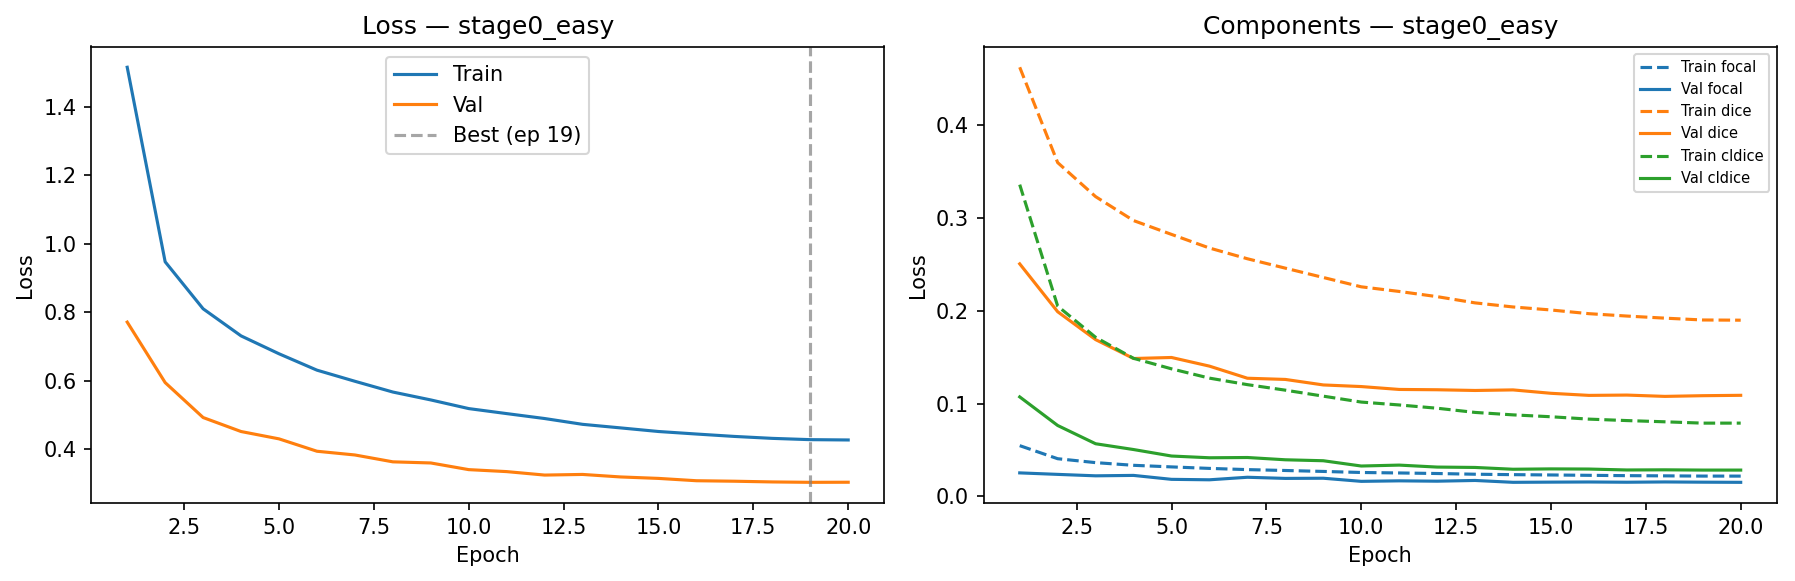
\includegraphics[width=\textwidth]{images/loss_stage0_easy.png}
%    \caption{Pannello di diagnostica dello \texttt{stage0\_easy}: loss totale, componenti e learning rate.}
%    \label{fig:loss_stage0}
%\end{figure}

%\begin{figure}[H]
%    \centering
%    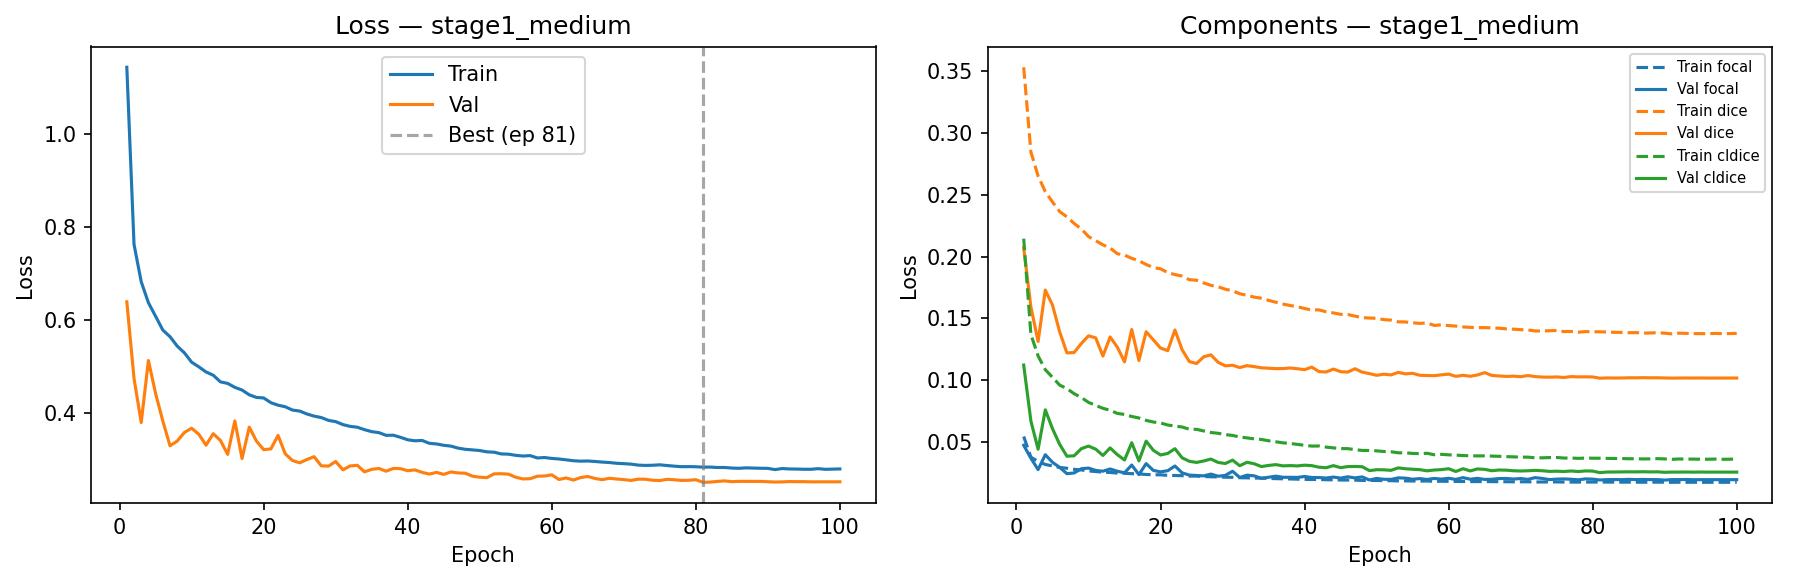
\includegraphics[width=\textwidth]{images/loss_stage1_medium.png}
%    \caption{Pannello di diagnostica dello \texttt{stage1\_medium}: loss totale, componenti e learning rate.}
%    \label{fig:loss_stage1}
%\end{figure}

%\begin{figure}[H]
%    \centering
%    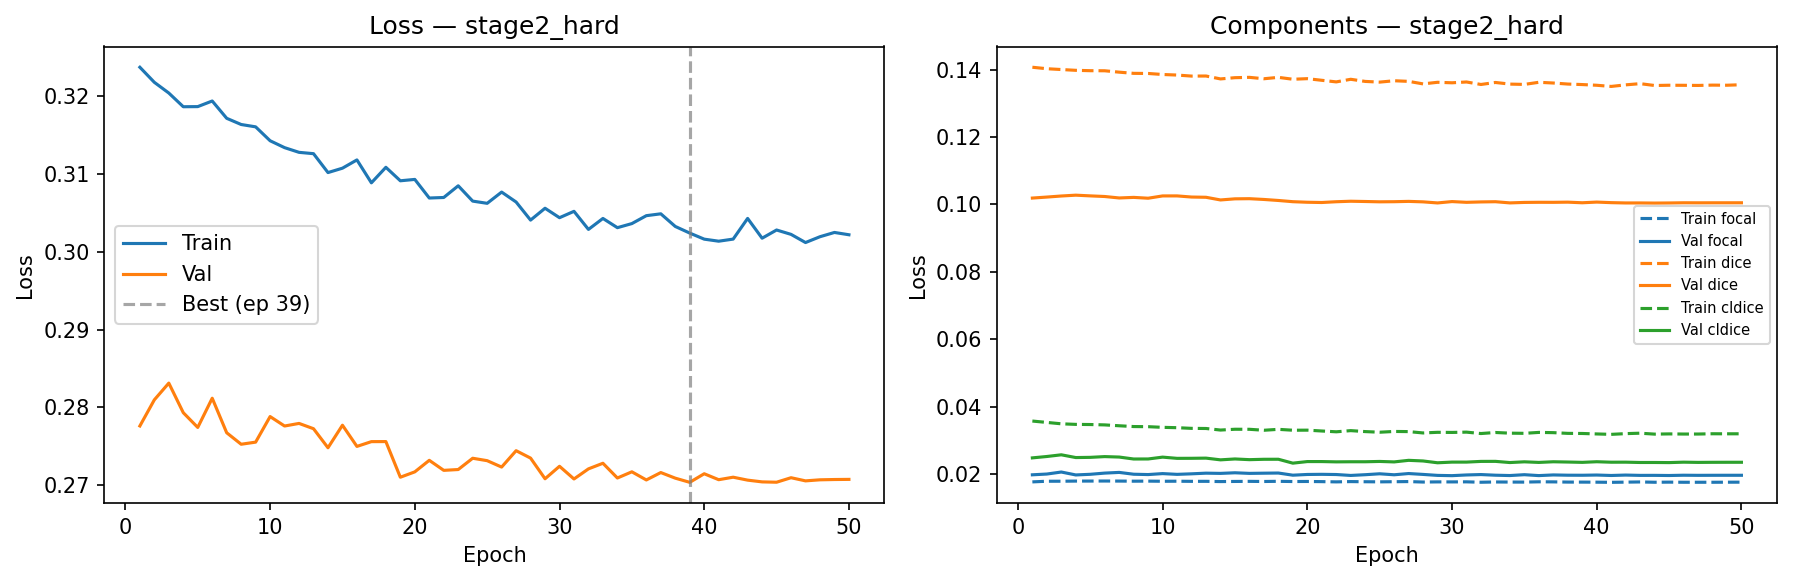
\includegraphics[width=\textwidth]{images/loss_stage2_hard.png}
%    \caption{Pannello di diagnostica dello \texttt{stage2\_hard}: loss totale, componenti e learning rate. La linea tratteggiata indica il best checkpoint all'epoca 34.}
%    \label{fig:loss_stage2}
%\end{figure}

% TODO: uncomment figures and re-enable this paragraph once loss plots are available
%Dalla Figura~\ref{fig:loss_stage2} emergono alcuni aspetti caratteristici dell'addestramento allo stage più difficile. La val loss converge significativamente più in basso della train loss: questo comportamento, apparentemente controintuitivo, è atteso in presenza di dropout e augmentation aggressiva applicata solo al training set — il modello vede immagini degradate durante l'addestramento ma viene valutato su immagini pulite. Il gap si riduce progressivamente man mano che il cosine annealing abbassa il learning rate, stabilizzando l'ottimizzazione. La componente Dice domina quantitativamente le altre per via della sua scala naturale nell'intervallo $[0, 1]$; le componenti Focal e clDice, pur di valore assoluto inferiore, esercitano un contributo proporzionalmente importante al gradiente complessivo grazie ai loro pesi nel calcolo della loss composita.

\subsection{Valutazione Finale sul Test Set}

Al termine di tutti gli stage, il modello viene valutato sul subset di test mantenuto separato durante tutto il training. Questo fornisce una stima non distorta delle prestazioni finali su dati mai visti, indipendente dalle scelte di iperparametri effettuate sulla base della val loss.

\subsection{Precisione Mista e Supporto Hardware}\label{sec:amp}

L'addestramento utilizza la \textbf{precisione mista automatica} (\textit{Automatic Mixed Precision}, AMP) tramite \texttt{torch.amp.GradScaler} e \texttt{torch.amp.autocast}. L'idea di fondo è che non tutte le operazioni di una rete neurale richiedono la stessa precisione numerica: le moltiplicazioni nei layer convoluzionali tollerano bene \texttt{float16} (16 bit), mentre l'aggiornamento dei pesi tramite gradiente richiede \texttt{float32} (32 bit) per non accumulare errori di arrotondamento.

Il contesto \texttt{autocast} gestisce questa distinzione automaticamente: avvolge il forward pass e il calcolo della perdita, e decide operazione per operazione quale precisione usare, senza che il codice debba specificarlo esplicitamente. Il vantaggio è duplice: le operazioni in \texttt{float16} occupano metà della VRAM e vengono eseguite più velocemente sui Tensor Core delle GPU moderne, che sono ottimizzati proprio per questo tipo di calcolo.

Il rischio della \texttt{float16} è però l'underflow dei gradienti: valori molto piccoli vengono arrotondati a zero e l'aggiornamento dei pesi si blocca. Il \texttt{GradScaler} risolve questo problema moltiplicando la perdita per un fattore di scala prima del backward pass — amplificando i gradienti per tenerli lontani dallo zero — e dividendo i gradienti stessi prima dell'aggiornamento dell'ottimizzatore, aggiustando dinamicamente il fattore di scala in base alla presenza di valori non finiti.

La mixed precision è abilitata automaticamente su CUDA e disabilitata su CPU e Apple Silicon (MPS), dove le istruzioni \texttt{float16} non offrono vantaggi o non sono supportate. Il rilevamento del dispositivo avviene in ordine di priorità: CUDA $\to$ MPS $\to$ CPU.

\section{Parametri di Configurazione}

\subsection{Selezione della Modalità}

\begin{itemize}
    \item \textbf{\texttt{--base\_dir}}: cartella con immagini ECG pulite; augmentation al volo, split 80/10/10 automatico.
    \item \textbf{\texttt{--base\_dir\_augmented}}: radice del dataset pre-augmentato, contenente \texttt{stage0\_easy}, \texttt{stage1\_medium}, \texttt{stage2\_hard}.
    \item \textbf{\texttt{--generator\_path}}: percorso alla directory \texttt{ecg-image-generator}; obbligatorio con \texttt{--base\_dir}.
\end{itemize}

I due argomenti \texttt{--base\_dir} e \texttt{--base\_dir\_augmented} sono mutuamente esclusivi.

\subsection{Parametri di Training}

\begin{itemize}
    \item \textbf{\texttt{--epochs}}: epoche per stage 1 e 2; default: \texttt{20}. Lo stage 0 usa sempre 5 epoche; lo stage 2 usa \texttt{--epochs // 2}.
    \item \textbf{\texttt{--batch}}: batch size; default: \texttt{8}.
    \item \textbf{\texttt{--encoder}}: backbone dell'encoder; default: \texttt{resnet50}. Opzioni comuni:
        \begin{itemize}
            \item \texttt{resnet50} — CNN, baseline generale affidabile
            \item \texttt{efficientnet-b5} — CNN, buon equilibrio tra precisione e memoria
            \item \texttt{mit-b2} — transformer, più leggero di \texttt{mit-b4}
            \item \texttt{mit-b4} — transformer, massima precisione, maggiore consumo di VRAM
        \end{itemize}
    \item \textbf{\texttt{--lr}}: learning rate per lo stage 0; default: \texttt{1e-4}.
    \item \textbf{\texttt{--lr\_medium}}: learning rate per lo stage 1; default: \texttt{1e-5}.
    \item \textbf{\texttt{--lr\_hard}}: learning rate per lo stage 2; default: \texttt{1e-6}.
    \item \textbf{\texttt{--workers}}: processi paralleli del DataLoader; default: \texttt{4}.
    \item \textbf{\texttt{--resize}}: risoluzione quadrata a cui ridimensionare le immagini; default: disabilitato.
    \item \textbf{\texttt{--freeze\_encoder}}: abilita l'unfreezing progressivo dell'encoder.
    \item \textbf{\texttt{--resume\_stage}}: riprende il training dallo stage specificato (0=easy, 1=medium, 2=hard); default: \texttt{0}.
    \item \textbf{\texttt{--load\_weights}}: percorso a un file \texttt{.pth} per inizializzare il modello prima del training.
    \item \textbf{\texttt{--val\_split}} / \textbf{\texttt{--test\_split}}: frazioni di validazione e test (solo con \texttt{--base\_dir\_augmented}); default: \texttt{0.1} ciascuna.
\end{itemize}

\section{Considerazioni sull'Occupazione di VRAM}

\begin{table}[H]
\centering
\caption{Stima del consumo di VRAM con mixed precision.}
\label{tab:extractor_vram}
\begin{tabular}{rrrr}
\hline
\textbf{Encoder} & \textbf{Risoluzione} & \textbf{Batch size} & \textbf{VRAM stimata} \\
\hline
\texttt{resnet50}      & $512 \times 512$   & 8 & $\sim 4$--$6$ GB \\
\texttt{resnet50}      & $1024 \times 1024$ & 4 & $\sim 8$--$12$ GB \\
\texttt{mit-b4}        & $512 \times 512$   & 8 & $\sim 8$--$10$ GB \\
\texttt{mit-b4}        & $1024 \times 1024$ & 4 & $\sim 16$--$20$ GB \\
\hline
\end{tabular}
\end{table}

Per configurazioni con VRAM limitata si raccomanda di utilizzare \texttt{resnet50} con \texttt{--resize 512} e batch size 4-8. La riduzione di risoluzione comporta una minore precisione sulla localizzazione dei tracciati più sottili, ma rimane accettabile per pipeline di pre-segmentazione.

\section{Visualizzazione e Post-processing delle Maschere}

\subsection{Visualizzazione per Stage}

Al termine di ogni stage di training, il modello produce automaticamente un pannello di visualizzazione su un sottoinsieme di immagini campione, specificabile tramite \texttt{--viz\_dir}. Il pannello affianca tre rappresentazioni per ogni immagine:

\begin{itemize}
    \item \textbf{Immagine originale:} il campione di input così come appare nel dataset, senza inversione né normalizzazione.
    \item \textbf{Heatmap di confidenza:} l'output del modello dopo la funzione sigmoid, visualizzato con colormap \textit{jet}. I valori vicini a 1 (rosso) indicano alta confidenza nella presenza del tracciato, quelli vicini a 0 (blu) indicano sfondo. La heatmap permette di identificare zone di incertezza — valori intermedi attorno a 0.5 — dove il modello esita tra tracciato e griglia.
    \item \textbf{Maschera binaria:} la heatmap sogliata a 0.5 (configurabile tramite \texttt{--threshold}), dopo il post-processing di rimozione delle macchie. I pixel a 1 rappresentano il tracciato predetto.
\end{itemize}

Confrontare i pannelli prodotti allo stage 0 e allo stage 2 permette di osservare visivamente il miglioramento portato dal curriculum learning: le maschere dello stage 0 tendono a includere porzioni di griglia come falsi positivi, mentre quelle dello stage 2 risultano più pulite grazie all'esposizione progressiva agli artefatti.

\subsection{Post-processing: Rimozione delle Macchie (\texttt{filter\_blobs})}

La maschera binaria prodotta dal modello può contenere falsi positivi corrispondenti a macchie d'inchiostro o blobs scuri presenti nell'immagine originale, che il modello può confondere con tracciati per via della loro intensità simile. La funzione \texttt{filter\_blobs()} applica un post-processing in due stadi per rimuoverli.

\paragraph{Stadio 1 — Rilevamento guidato dall'immagine.} Viene applicato un blur gaussiano con sigma elevato (default: 25 px) all'immagine originale in scala di grigi. Le linee sottili del tracciato ECG (larghezza tipica 2–8 px) svaniscono nel processo di sfocatura, mentre le macchie d'inchiostro di grandi dimensioni rimangono scure. Le regioni in cui il valore dell'immagine sfocata è inferiore a una soglia (default: 150 su scala 0–255) vengono identificate come macchie e rimosse dalla maschera binaria.

\paragraph{Stadio 2 — Pulizia tramite distance transform.} Per catturare eventuali regioni spesse non rilevate dallo stadio 1, viene calcolata la \textit{distance transform} della maschera pulita: ad ogni pixel viene assegnata la distanza in pixel dal bordo più vicino della regione predetta. Le regioni con distanza superiore a una soglia (default: 15 px) vengono considerate troppo spesse per essere tracciati ECG — la cui semi-larghezza tipica è di 2–8 px — e le loro aree centrali vengono espanse tramite dilatazione morfologica e rimosse dalla maschera. Infine, le componenti connesse con area inferiore a 20 pixel vengono eliminate come rumore residuo.

\section{Detection Head Multi-task per la Localizzazione dei Lead}
\label{sec:detection_head}

Il flag \texttt{--detection} estende il modello base con una \textbf{testa di detection multi-task} che, in aggiunta alla segmentazione, predice per ciascuno dei 12 lead ECG standard: (1) se il lead è presente nell'immagine, (2) la regione del tracciato e (3) la regione dell'etichetta testuale, entrambe come bounding box orientati.

\subsection{Architettura della Detection Head}

Quando \texttt{--detection} è attivo, la classe \texttt{smp.Unet} viene sostituita da \texttt{ECGMultiTaskModel}, che condivide l'encoder e il decoder con il task di segmentazione e aggiunge una \texttt{DetectionHead} collegata al collo di bottiglia dell'encoder.

La scelta cruciale riguarda \textit{come} condensare le feature maps spaziali del bottleneck — di forma \texttt{(B, C, H, W)} — in un vettore da passare all'MLP. Un \textit{global average pooling} collasserebbe tutte le dimensioni spaziali in un unico valore per canale, distruggendo le informazioni su \textit{dove} si trovano i lead nell'immagine e costringendo il modello a predire bounding box allineati agli assi. Per preservare la struttura spaziale, la testa utilizza invece un \textbf{pooling separato per strisce orizzontali e verticali}:

\begin{enumerate}
    \item Una convoluzione $1\times1$ riduce i canali da $C$ a 256, seguita da batch normalization e ReLU.
    \item Un \textit{row-strip pooling} divide l'asse verticale in 8 fasce e ne calcola la media lungo l'asse orizzontale, producendo un vettore di dimensione $256 \times 8$.
    \item Un \textit{col-strip pooling} divide l'asse orizzontale in 8 fasce e ne calcola la media lungo l'asse verticale, producendo un vettore di dimensione $256 \times 8$.
    \item I due vettori vengono concatenati (dimensione totale 4096) e passati a un MLP con uno strato nascosto da 512 neuroni, ReLU e dropout (0.3).
    \item Il layer finale produce $12 \times 13$ logit: 1 (presenza) $+ 6$ (bounding box lead) $+ 6$ (bounding box etichetta) per ognuno dei 12 lead.
\end{enumerate}

\subsection{Rappresentazione OBB (Oriented Bounding Box)}

Un \textbf{bounding box allineato agli assi} (AABB, \textit{Axis-Aligned Bounding Box}) è il rettangolo minimo che contiene un oggetto i cui lati sono paralleli agli assi dell'immagine: è descritto da soli 4 parametri (coordinate del centro, larghezza, altezza) ma non può rappresentare oggetti inclinati senza includervi ampio sfondo vuoto. Per oggetti orientati — come le regioni dei lead ECG, che possono essere inclinati quando l'immagine è stata ruotata in augmentation — questa approssimazione introduce un errore di localizzazione sistematico.

Un \textbf{oriented bounding box} (OBB) risolve il problema aggiungendo un grado di libertà: l'angolo di rotazione $\theta$ del rettangolo rispetto all'orizzontale. Un OBB è quindi il rettangolo minimo che contiene l'oggetto senza il vincolo di allineamento agli assi, e può rappresentare fedelmente regioni inclinate di qualsiasi angolo.

\begin{figure}[H]
    \centering
    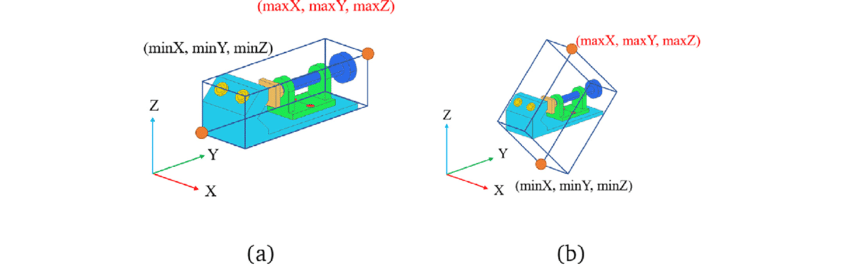
\includegraphics[width=0.8\textwidth]{images/obb_vs_aabb.png}
    \caption{Confronto tra AABB (tratteggiato) e OBB (continuo) su una regione di lead ECG inclinata. L'AABB include una larga porzione di sfondo, mentre l'OBB aderisce alla forma reale del tracciato.}
    \label{fig:obb_vs_aabb}
\end{figure}

In questa implementazione i bounding box vengono rappresentati come OBB con \textbf{6 parametri} anziché le 8 coordinate libere dei quattro angoli:

\[
    \text{OBB} = \bigl[c_x,\; c_y,\; w,\; h,\; \sin(2\theta),\; \cos(2\theta)\bigr]
\]

dove $(c_x, c_y)$ è il centro normalizzato, $w$ e $h$ sono larghezza e altezza normalizzate (con $w \geq h$ per convenzione, rendendo $\theta$ l'angolo dell'asse più lungo), e $\theta$ è l'angolo di rotazione rispetto all'orizzontale.

La scelta di 6 parametri rispetto agli 8 delle coordinate libere non è solo una questione di compattezza: supervisionare 8 coordinate indipendenti non impone al modello alcun vincolo geometrico, per cui può predire quadrilateri degeneri che non sono rettangoli. La parametrizzazione OBB garantisce per costruzione che l'output sia sempre un rettangolo valido.

\paragraph{Codifica a doppio angolo.} La scelta di codificare l'angolo come $\sin(2\theta)/\cos(2\theta)$ anziché come $\theta$ direttamente — o come $\sin(\theta)/\cos(\theta)$ — è motivata dalla simmetria dei rettangoli: un rettangolo ruotato di $180°$ è geometricamente identico all'originale. Se si utilizzasse la codifica diretta $\sin(\theta)/\cos(\theta)$, per uno stesso rettangolo esisterebbero due valori target ugualmente validi ($\theta$ e $\theta + 180°$), e la rete riceverebbe un segnale di addestramento ambiguo — in certi batch verrebbe spinta verso $\theta$, in altri verso $\theta + 180°$, ostacolando la convergenza. Usando $2\theta$, i due angoli equivalenti vengono mappati allo stesso punto nel piano $(\sin, \cos)$, eliminando l'ambiguità e rendendo il target univoco.

I parametri geometrici $(c_x, c_y, w, h)$ vengono predetti applicando una sigmoid ai logit corrispondenti, ottenendo valori in $(0,1)$ coerenti con le coordinate normalizzate; i parametri angolari $(\sin(2\theta), \cos(2\theta))$ vengono predetti applicando una tanh, ottenendo valori in $(-1,1)$ coerenti con il codominio delle funzioni trigonometriche. La conversione ai quattro angoli del rettangolo avviene tramite la funzione \texttt{obb\_to\_corners()} a tempo di inferenza.

\subsection{Funzione di Perdita per il Rilevamento}

La perdita totale è la somma della perdita di segmentazione e della perdita di detection:

\[
    \mathcal{L}_{\text{tot}} = \mathcal{L}_{\text{seg}} + \mathcal{L}_{\text{det}}
\]

La perdita di detection è a sua volta composta da tre termini:

\[
    \mathcal{L}_{\text{det}} = w_p\,\mathcal{L}_{\text{BCE}}(\text{presenza}) + w_b\,\mathcal{L}_{\text{SL1}}(c_x,c_y,w,h) + w_a\,\mathcal{L}_{\text{MSE}}(\sin 2\theta, \cos 2\theta)
\]

Tutti i termini geometrici e angolari sono calcolati solo sui lead effettivamente presenti nell'immagine (masking tramite il vettore di presenza ground truth). La Smooth-L1 viene usata per le coordinate geometriche per la sua robustezza agli outlier; la MSE è preferibile per i componenti angolari perché il codominio è limitato e si vuole una penalizzazione simmetrica intorno all'errore zero.

Le immagini prive di file JSON di annotazione contribuiscono solo alla perdita di segmentazione: la perdita di detection viene saltata per quei campioni del batch.

\subsection{Conversione Ground Truth e Inferenza}

A tempo di caricamento, i bounding box corner forniti dal generatore (formato $[[x_1,y_1],[x_2,y_2],[x_3,y_3],[x_4,y_4]]$) vengono convertiti in OBB tramite la funzione \texttt{corners\_to\_obb()}: si calcolano centro, vettori degli spigoli e angolo dell'asse più lungo, normalizzando le coordinate per larghezza e altezza dell'immagine.

Quando l'augmentation include rotazione (\texttt{--rotate}), le coordinate dei corner vengono ruotate dall'augmentatore \texttt{get\_augment()} prima della conversione in OBB, garantendo la coerenza tra immagine augmentata e annotazioni.

A tempo di inferenza, \texttt{test\_and\_visualize\_masks.py} converte le OBB predette in coordinate pixel tramite \texttt{obb\_to\_corners()} e le disegna come poligoni quadrilateri sull'immagine originale, supportando la visualizzazione di bounding box ruotati.

\subsection{Stage di Fine-tuning della Detection Head}
\label{sec:det_finetune}

L'addestramento congiunto di segmentazione e detection presenta un problema strutturale: la perdita di segmentazione domina numericamente quella di detection, assorbendo la quasi totalità del segnale di gradiente. La \texttt{DetectionHead}, inizializzata casualmente, riceve un aggiornamento troppo debole per convergere efficacemente durante i tre stage del curriculum.

Per risolvere questo problema, al termine dello \texttt{stage2\_hard} viene eseguito automaticamente un quarto stage dedicato esclusivamente alla detection, attivato dalla presenza del flag \texttt{--detection}. Durante questo stage:

\begin{itemize}
    \item L'intera U-Net — encoder, decoder e testa di segmentazione — viene \textbf{congelata}: i suoi pesi non ricevono aggiornamenti.
    \item Solo i parametri della \texttt{DetectionHead} rimangono addestrabili.
    \item Il learning rate viene reimpostato al valore \texttt{--det\_finetune\_lr} (default $10^{-3}$), significativamente più alto del $10^{-6}$ usato nello \texttt{stage2\_hard}, poiché la testa deve apprendere da zero anziché effettuare un fine-tuning di precisione.
    \item L'ottimizzatore e il cosine annealing scheduler vengono reinizializzati per questo stage.
\end{itemize}

Il risultato è che il $100\%$ della capacità computazionale del gradiente viene dedicata alla regressione dei bounding box, senza competizione con il task di segmentazione. I pesi migliori vengono salvati in \texttt{ecg\_attention\_unet\_det\_finetune.pth}.

È possibile eseguire solo questo stage su un checkpoint di segmentazione già addestrato, saltando i tre stage del curriculum tramite \texttt{--resume\_stage 3}:

\begin{minted}{bash}
python extractor.py \
  --base_dir /data/ecg_clean \
  --load_weights ecg_attention_unet_stage2_hard.pth \
  --resume_stage 3 \
  --detection --det_finetune_epochs 30 --det_finetune_lr 1e-3
\end{minted}

\section{Utilità per la Preparazione del Dataset}

Il modulo include lo script \texttt{clean\_dataset.py}, un'utilità di pre-processing per verificare l'integrità delle coppie immagine/maschera prima di avviare il training. Lo script scansiona ricorsivamente la directory del dataset, tenta di caricare ogni immagine e la corrispondente maschera tramite PIL, e segnala le coppie corrotte o troncate.

Di default opera in modalità \textit{dry run}: riporta i file problematici senza eliminarli. Con il flag \texttt{--delete} rimuove fisicamente entrambi i file della coppia corrotta. Questo passaggio è consigliato prima di ogni sessione di training per evitare che immagini illeggibili interrompano il DataLoader o producano batch con maschere nulle non rilevate.
